\documentclass[tikz,border=5mm]{standalone}
\usepackage{tikz}
\usepackage{amsmath}
\usetikzlibrary{positioning, calc, arrows.meta, shapes.geometric, fit}

%% Fonts
\usepackage{helvet}
\renewcommand{\familydefault}{\sfdefault}
\usepackage{sansmath}
\sansmath
\DeclareSymbolFont{sfoperators}{OML}{cmm}{m}{it}
\DeclareMathSymbol{\Delta}{\mathalpha}{sfoperators}{"01}

%% Colors
\definecolor{colour_ml}{HTML}{440154}
\definecolor{colour_exp}{HTML}{35b779}
\definecolor{colour_ie}{HTML}{31688e}
\definecolor{colour_residual}{HTML}{ff991c}

\begin{document}
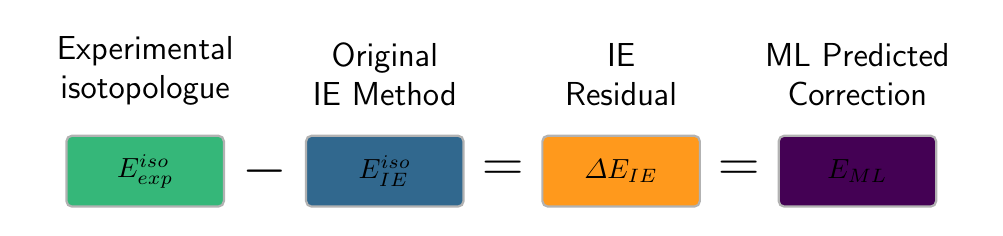
\begin{tikzpicture}[
    font=\sffamily,
    box/.style={rectangle, draw=gray!60, thick, rounded corners=2pt,
                minimum height=0.9cm, minimum width=2cm, align=center},
    arrow/.style={-{Latex[length=2mm]}, thick, gray!70},
    ML_style/.style={fill=colour_ml},
    exp/.style={fill=colour_exp},
    ie_style/.style={fill=colour_ie},
    residual/.style={fill=colour_residual}
]

% Main equation boxes
\node[box, exp] (iso) {$E_{exp}^{iso}$};
\node[font=\huge, right=0.1cm of iso] (minus) {$-$};
\node[box, ie_style, right=0.1cm of minus] (ie) {$E_{IE}^{iso}$};
\node[font=\huge, right=0.1cm of ie] (equals) {$=$};
\node[box, residual, right=0.1cm of equals] (resid) {$\varDelta E_{IE}$};
\node[font=\huge, right=0.1cm of resid] (equals2) {$=$};
\node[box, ML_style, right=0.1cm of equals2] (ML) {$E_{ML}$};

% Labels above
\node[above=0.25cm of ie, font=\large, text width=2.75cm, align=center] 
     {Original\\IE Method};
\node[above=0.25cm of iso, font=\large, text width=2.75cm, align=center] 
     {Experimental\\isotopologue};
\node[above=0.25cm of resid, font=\large, text width=2.75cm, align=center]
     {IE\\Residual};
\node[above=0.25cm of ML, font=\large, text width=2.75cm, align=center]
     {ML Predicted\\Correction};

\end{tikzpicture}
\end{document}